\label{ternary}

%бедно и непонятно, исправить обязательно. Может подумать о картинке в пример, дабы было нагляднее. 

В качеcтве операторов для данного алгоритма введем следующие несмещенные операторы: 
\begin{itemize}
   \item $flipOne(a)$~--- изменение одного бита
   \item $flip'(a, b)$~--- изменить один бит из совпадающего суффикса
   \item $xor3(a,b,c)$~--- оператор исключающего ИЛИ для трех векторов 
\end{itemize}

(вставить формальное доказательство, что xor3 -> несмещенный)

Тогда рассмотрим следующий алгоритм: 
\begin{algorithm}[H]
\caption{Тернарный алгоритм}\label{lst1}
\begin{algorithmic}
        \State $q_0 \leftarrow \textrm{random}$
        \State $s_1 \leftarrow flipOne(q_0)$
		\While{true}
	        \State $s_2 \leftarrow flip'(q_0, s_1)$
            \State $t_2 \leftarrow xor3(q_0,s_1,s_2)$
            \State $s_3 \leftarrow flip'(q_0, t_2)$
            \State $t_3 \leftarrow xor3(q_0,s_2,s_3)$
            \State \ldots
		\EndWhile
\end{algorithmic}
\end{algorithm}

Таким образом формируется полное пространство поиска: 
\begin{example}
Пример генерации пространства для $q_0 = [000...000]$  \\
    $q_0$ = \{00000..0000\} \\
    $s_1$ = \{00000..0001\} \\
    $s_2$ = \{00000..0010\} \\
    $t_2$ = \{00000..0011\} \\
    $s_3$ = \{00000..0100\} \\
    $t_3$ = \{00000..0101\} \\
    ... \\
    $t_k$ = \{10000..0000\} \\
    ... \\
\end{example}

\begin{figure}[H]
\centering
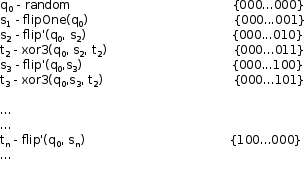
\includegraphics[height=7cm]{pic/tern0.png}
\caption{Пример генерации множества поиска для $q_0$}\label{fig2}
\end{figure}

%Размазано и непонятно. Переписать точно.
Таким образом пошагово генерируется все множество поиска без повторов. Сложность такого алгоритма равняется $O(\frac{2^n + 1}{2})$, 
что равняется времени перебора всех векторов без повторов. Таким образом, верхняя и нижняя оценки сложности алгоритма совпадают. 

%Что-то вроде примера 
Рассмотрим класс некоторых задач, таких что экземпляром данной задачи является битовая строка из пространства поиска, размера $2^n$ от длины строки $n$. При этом у задачи существует единственный 
глобальный оптимум (при этом  наличие других оптимумов не важно). К таким задачам относится, например, \textsc{OneMax}.

Задачи данного класса должны имееть примерно такой тип:
$$P = \{..2^n \textrm{instanses with bitwise} ... \}$$

Пусть существует оптимальный детерминированный алгоритм, который в среднем по всем экзеплярам выдает время работы T, при этом алгоритм не является black-box алгоритмом. 

Пусть $q_0$ - рандомизированный вектор, подающийся на вход алгоритму.

Тогда дерево решений данного алгоритма выглядит так: 

\begin{figure}[H]
\centering
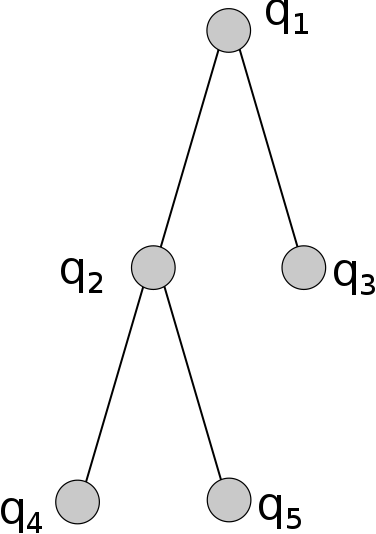
\includegraphics[height=5cm]{pic/graph1.png}
\caption{Дерево решений детерминированного алгоритма}
\end{figure}

Возьмем произвольный вектор $z$ и проксорим его с каждым решением из приведенного выше дерева. Таким образом все равно получится оптимальный детерминированны алгоритм, решающий данную задачу, но выглядеть 
он будет уже иначе, допустим, так: 

\begin{figure}[H]
\centering
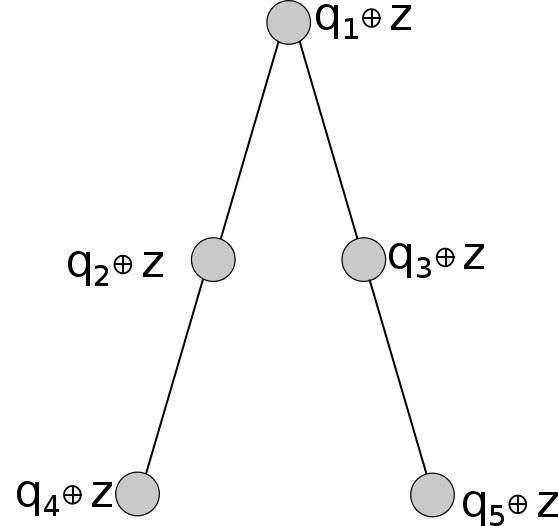
\includegraphics[height=5cm]{pic/graph2.png}
\caption{Дерево решений другого оптимального алгоритма}
\end{figure}

Тогда моделизируем процесс. 
$q_0$~--- так и остается рандомизированным вектором.
Исходя из дерева решений, известно, что переход в дереве от $q_1 \to q_2$ является не более чем изменением одного бита. 

Так как при моделировании аллгоритма с тернарным оператором мы можем сгенерировать множество векторов, показанное в примере 3, то мы умеем получать переходы при изменении от одного бита к другому. 

Тогда $z$ больше не просто случайный вектор, а $z = q_0 \oplus q_1 $, что, таким образом, и будет являться переходом $q_1 \to q_2$ в дереве решений. А так как при применения $\oplus$ к вершине 
изначального дерева, также получается детерминированный алгоритм, то учитывая построение множества, тогда несмщенный black-box алгоритм будет работать за $\leq(n + 1)T$
